\chapter{Design}

\begin{chapterabstract}
Selection of used technologies, establishment of the domain model, and initial design of the user interface layout.
\end{chapterabstract}


%---------------------------------------------------------------
\section{Technologies}
%---------------------------------------------------------------

Choosing the appropriate technologies is crucial and will have a significant impact on the overall effectiveness and excellence of the developed solution. Selecting technologies requires assessing different technological choices based on all the factors that will enable them to meet the requirements outlined in the preceding chapter. The right technology stack can also decrease the time spent on development, minimize costs, and ensure the solution remains relevant in the future.


% - - - - - - - - - - - - - - - - - - - - - - - - - - - - - - -
\subsection{Platform}
% - - - - - - - - - - - - - - - - - - - - - - - - - - - - - - -

In considering the foundation for the modular product configurator, given the multiplatform requirement (\hyperref[itm:NF1]{NF1}), two distinct development approaches were evaluated: applications specifically designed for desktop and mobile platforms and a web application.

Desktop and mobile applications can provide a better overall experience tailored to the specific platform and potentially be more performant as they can utilize the hardware better; however, in this case, they come with serious drawbacks. Having multiple applications that are designed for different devices would increase the amount of maintenance and development work required because each version would need to be managed (at least partially) separately. Furthermore, accessibility for users would be dramatically diminished since they would need to download and install the application prior to using it and subsequently manage any updates that may arise.

Developing separate desktop and mobile applications presents such significant challenges that the disadvantages far outweigh the advantages; therefore, a web application was selected for its better alignment with the project's requirements (this is also consistent with the norm in this space, as the majority of existing solutions that were analyzed in the previous chapter are web-based). There are also several key factors in favor of this solution: it can be accessed from any device with an internet connection and web browser, it is cost-effective as it possibly utilizes existing website infrastructure, and it has streamlined maintenance needs. The application will be client-side and focused on the front-end, as that is where the configuration process will be happening.


% - - - - - - - - - - - - - - - - - - - - - - - - - - - - - - -
\subsection{3D visualization technology} \label{section:3Dvistech}
% - - - - - - - - - - - - - - - - - - - - - - - - - - - - - - -

To fulfill the requirement of 3D visualization (\hyperref[itm:F1]{F1}), a library will have to be used that will allow 3D graphics to be rendered in the browser. However, the range of options for this particular technology is quite restricted.

Historically, the integration of 3D graphics required the use of external plugins, primarily Adobe Flash Player. The evolution of web standards, particularly the introduction of HTML5, has revolutionized this aspect, and it is now possible to render 3D graphics directly in the browser, eliminating the necessity for any plugin. \cite{Parisi2014}

WebGL (Web Graphics Library) is a standard 3D graphics API for web browsers. It is based on OpenGL ES and can be used inside the HTML canvas element. WebGL is supported in all major desktop and mobile browsers.\footnote{WebGL browser support details: \url{https://caniuse.com/webgl}} It is utilized using C-like shading language (OpenGL Shading Language) and JavaScript. \cite{Parisi2012}

Currently, there are no significant alternatives to WebGL. WebGPU aims to be a successor to WebGL; however, as of February 2024, it is in a state of ongoing development and has not yet been finalized or supported in web browsers.\footnote{WebGPU browser support details: \url{https://caniuse.com/webgpu}} \cite{WebGPU}


%______________________________________________________________
\subsubsection{WebGL framework} \label{section:WebGL}

Direct WebGL programming is very powerful and offers fine-grain control, necessitating extensive code to be written in both JavaScript and its shader language. Fortunately, there are several frameworks built on top of WebGL that provide high-level abstractions and access. These frameworks can significantly reduce the amount of code required to achieve what would otherwise take hundreds of lines when using bare WebGL, often condensing it into just a few lines. \cite{Parisi2014}

Three.js was selected from a range of frameworks, including Babylon.js and PixiJS, that are designed to streamline the process of developing in WebGL. This decision was made after considering several important factors.
Three.js is considered an undisputed leader in this category, having the biggest community support, which can be evidenced by its popularity and the volume of contributions on GitHub.\footnote{Three.js GitHub: \url{https://github.com/mrdoob/three.js}} It is also open source, published under the MIT license, offering great freedom in development and distribution. Furthermore, Three.js uses the best practices of 3D graphics; it is lightweight, easy to use, cross-platform, and contains many prebuilt assets. \cite{Parisi2014} \cite{ThreeJs} \cite{BabylonJs} \cite{PixiJS}


% - - - - - - - - - - - - - - - - - - - - - - - - - - - - - - -
\subsection{Front-end framework}
% - - - - - - - - - - - - - - - - - - - - - - - - - - - - - - -

Leveraging front-end frameworks significantly enhances the development of web applications by addressing common front-end challenges. These frameworks often provide a structured approach for creating maintainable and reusable components, optimizing data manipulations, employing common design patterns, and ensuring that the user interface remains in sync with the underlying state. Various frameworks and libraries are available, such as React, Vue.js, or Angular, each with different benefits and drawbacks. The choice of which framework to use often involves complex decision making, influenced by specific project needs, team skills, and the unique characteristics of each framework. \cite{Gimeno2018} \cite{Pekarsky2020}

For this solution, the decision has been greatly influenced by the selection of \hyperref[section:WebGL]{WebGL framework}, Three.js. The React Three Fiber (R3F) library offers a seamless integration of Three.js into the React ecosystem. R3F is a React renderer, enabling the direct use of Three.js components as React components. The integration is optimized, with the Three.js components rendered outside React's rendering process, therefore, having minimal overhead. Moreover, it is comprehensive, meaning that all Three.js features are exposed and accessible using this library. \cite{R3F}

In addition, the Drei library, built on top of R3F, introduces a collection of useful components, abstractions, and helpers. These additions streamline the development with Three.js and React even more. \cite{Drei}

These libraries make React an attractive choice for this project. To see how the code differs when aiming to achieve similar objectives, refer to \autoref{listing:threejs} for the plain Three.js version and \autoref{lisiting:r3f} for the R3F version, both creating a simple 3D red cube.

React is a user interface library created at Facebook in 2011, but soon after became open source. React has gained widespread acclaim across many projects and has been continually developed since its inception. It emphasizes component-based architecture, where reactive components are written in JavaScript (or TypeScript) combined with HTML-like markup code, facilitating the creation of dynamic user interfaces. \cite{Banks2020}

React itself is just a user interface library that lacks more sophisticated functionalities, such as routing. There are several frameworks compatible with React, such as Next.js or Gatsby.js, which offer advanced features like caching, routing, server-side rendering, search engine optimization, and more. However, because the dynamic content of this web application is highly influenced by user interactions, the solution would not benefit from these frameworks. \cite{Eze2023} Therefore, the decision was made to maintain simplicity, opting for the utilization of select libraries for advanced features rather than complex frameworks. Prioritizing speed, simplicity, and minimal configuration requirements, Vite.js has been chosen as the build tool and development server. \cite{Said2023}


%______________________________________________________________
\subsubsection{CSS framework}

The development of a product configurator requires custom components. To define the styles of these custom designs, it will be necessary to utilize CSS (Cascading Style Sheets).

TailwindCSS is a utilitfy-first CSS framework. It enables the creation of custom designs using predefined CSS utility classes, directly applicable in the React markup language, eliminating the necessity of manually writing CSS. It is highly and simply customizable, has comprehensive and illustrative documentation, and makes it easy to create responsive designs. The framework allows for a fast development process, however, it needs to be integrated carefully, as the direct combination of style classes with the rest of the code of the component can make the codebase look very disorganized. \cite{TailwindCSS}

It was chosen for this project as a good balance between a fully custom solution and predefined components, for its ability to accelerate the development process and to help fulfill the requirement \hyperref[itm:NF2]{NF2}.


% - - - - - - - - - - - - - - - - - - - - - - - - - - - - - - -
\subsection{Programming languages}
% - - - - - - - - - - - - - - - - - - - - - - - - - - - - - - -

The selection of programming language is predetermined by the already chosen technologies and libraries, necessitating the use of React markup and JavaScript in some form.

Fortunately, with Vite.js's ability to transpile TypeScript to JavaScript, and given that type declarations are exported from the chosen JavaScript libraries, TypeScript can also be used. \cite{Said2023}

TypeScript is a programming language created by Microsoft that extends JavaScript by implementing strong typing. Strong typing helps detect bugs during development, reduce runtime errors, and improve overall code quality. It also allows for tighter integration with code editors, enabling features such as autocompletion or inline documentation. All code written in TypeScript is transpilable to JavaScript, which means that it is compatible with existing libraries and frameworks. \cite{TypeScript}

Given these advantages, TypeScript will be used in this project in place of JavaScript, ensuring a maintainable, high-quality codebase.


% - - - - - - - - - - - - - - - - - - - - - - - - - - - - - - -
\subsection{Additional libraries}
% - - - - - - - - - - - - - - - - - - - - - - - - - - - - - - -

To enhance the functionality in a way that the frameworks described above do not support natively, several additional libraries will be used in the solution.

%______________________________________________________________
\subsubsection{Routing} \label{section:react-router}

To improve the application's user experience with navigable URLs, allowing redirection, linking, or bookmarking pages, the use of a routing library is essential, as in an SPA, all content is served on a single address by default. For React, the leading library for routing is React-Router, which will be utilized for this purpose in this solution. This library has been chosen for its widespread use and robustness. Its use promises that the application supports dynamic and user-friendly navigation. \cite{Ganatra2018}

%______________________________________________________________
\subsubsection{Language support} \label{section:i18n}

To address the requirement of user interface text customization (\hyperref[itm:F15]{F15}) and multilingual support (\hyperref[itm:NF8]{NF8}), an internationalization and localization library is essential. Such a library enables the dynamic sourcing of user-interface texts from separate files according to the application's current settings. Consequently, on the basis of the extensive set of features and extensions offered, the i18next internationalization framework was chosen for this project. \cite{Krukowski2023}

%______________________________________________________________
\subsubsection{State management}

State management is a critical element of React applications that links the internal state directly to the user interface. Although React offers a basic mechanism by default, complex applications highly profit from a sophisticated state management library that manages state updates and interface redraws in a comprehensive manner. \cite{Ceddia2021}

Although there are numerous different state management libraries, each with its advantages and disadvantages (such as Zustand, Redux, MobX, etc.), for this project, Valtio has been chosen. Valtio stands out for its extremely minimalistic API, while being very flexible with data structures. It uses proxies and allows direct mutations, making the handling of state as intuitive as working with regular JavaScript (or TypeScript) objects. This makes Valtio highly beneficial for this application, as it will simplify mapping the changing state to 3D objects, which will be necessary to fulfill the 3D preview requirement \hyperref[itm:F1]{F1}). \cite{Adepoju2023}

%______________________________________________________________
\subsubsection{Validation} \label{section:zod}

To guarantee the integrity and structure of the loaded data, together with values that adhere to specified constraints, validation is crucial. Validation libraries have been designed for this purpose, and in this project, Zod has been chosen as the data validation library. Zod allows the inference of TypeScript types directly from the created data schemas, meaning a single schema definition can be used for parsing as well as type checking. Furthermore, Zod's is also very lightweight, and its powerful yet straitforward API for schema definition makes it an excellent choice for this task. \cite{Bhimani2023}


% - - - - - - - - - - - - - - - - - - - - - - - - - - - - - - -
\subsection{Development tooling}
% - - - - - - - - - - - - - - - - - - - - - - - - - - - - - - -

The effectiveness and resilience of the development process depends on the selection of development tools. These tools not only simplify code creation, but also help ensure code quality, version control, and improve efficiency in collaborative work.

%______________________________________________________________
\subsubsection{Version control}

Version control plays a crucial role in modern software development, allowing developers to track changes to source code over time. For this project, Git has been chosen as the version control system due to its widespread adoption and robust feature set. Git is a distributed system that allows for easy collaboration with other developers, as well as the creation of independent adaptations of the codebase through forking, all while preserving a connection to the original repository for future updates or integrations. In this way, a unique version of the application codebase can be tailored to meet specific business needs effectively.  \cite{Ponuthorai2022}

GitLab is a DevOps platform that is used to host Git repositories, offering a wide range of features. The primary benefit for this project lies in its CI/CD pipelines, which can be used for automated testing, linting, and building of the project. This automation speeds up the development process. \cite{GitLab}

Conventional Commits is a convention for naming Git commit messages in a descriptive form, creating rules that communicate the scope of changes and allow the creation of further automations on top of them. This convention will be used to ensure order and clarity in the Git repository. \cite{ConventionalCommits}

To enforce the use of conventions in commits, Husky, a tool for utilizing Git hooks, will be integrated into the development workflow. Husky allows for the setup of actions that are triggered at specific points in the Git lifecycle. This way, the project can automatically lint commit messages to ensure that they follow the Conventional Commits format, as well as check contents of the commits. \cite{Husky}

%______________________________________________________________
\subsubsection{Package manager}

To streamline the process of managing the dependencies of the project, npm has been selected as the package manager due to its wide adoption and compatibility within the ecosystem. \cite{Abramowski2022}

%______________________________________________________________
\subsubsection{Formatters}

For ensuring code consistency and style guidelines adherence, especially when working with TypeScript, due to the loose nature of the language, linters and code formatters need to be used.

ESLint will be used as a linter to help identify and fix problems in TypeScript code, removing problematic patterns, promoting best practices and code consistency. \cite{Gupta2021}

Prettier will automatically format the code to meet style guidelines, making it easy to read and reducing formatting discrepancies. \cite{Wojtasinski2023}


%---------------------------------------------------------------
\section{Domain model} \label{section:domain-model}
%---------------------------------------------------------------

Before implementation, an important part of the design process is the description of the domain model. This outlines the concepts with which the tool will work and defines the entities' interactions, establishing an important context that serves as a foundation for building the toolkit. A Unified Modeling Language (UML) diagram can easily represent the domain model. \cite{Wlaschin2018}

The UML diagram that illustrates the domain model of the entities related to the proposed toolkit is presented in \autoref{fig:domain-model}. This model serves as a blueprint for the architecture of the system, outlining a coherent structure that aligns with the project objectives described in the previous chapters. 

The model domain presents a structure of product and component specifications contained in a catalog, the dependencies between different entities, and illustrates the progression from generic specifications to concrete user configurations. This model aims to offer a clearer insight into the design rationale behind the tool, highlighting the transition from abstract specifications to customized user-driven outcomes.

\begin{landscape}
\begin{figure}
\centering
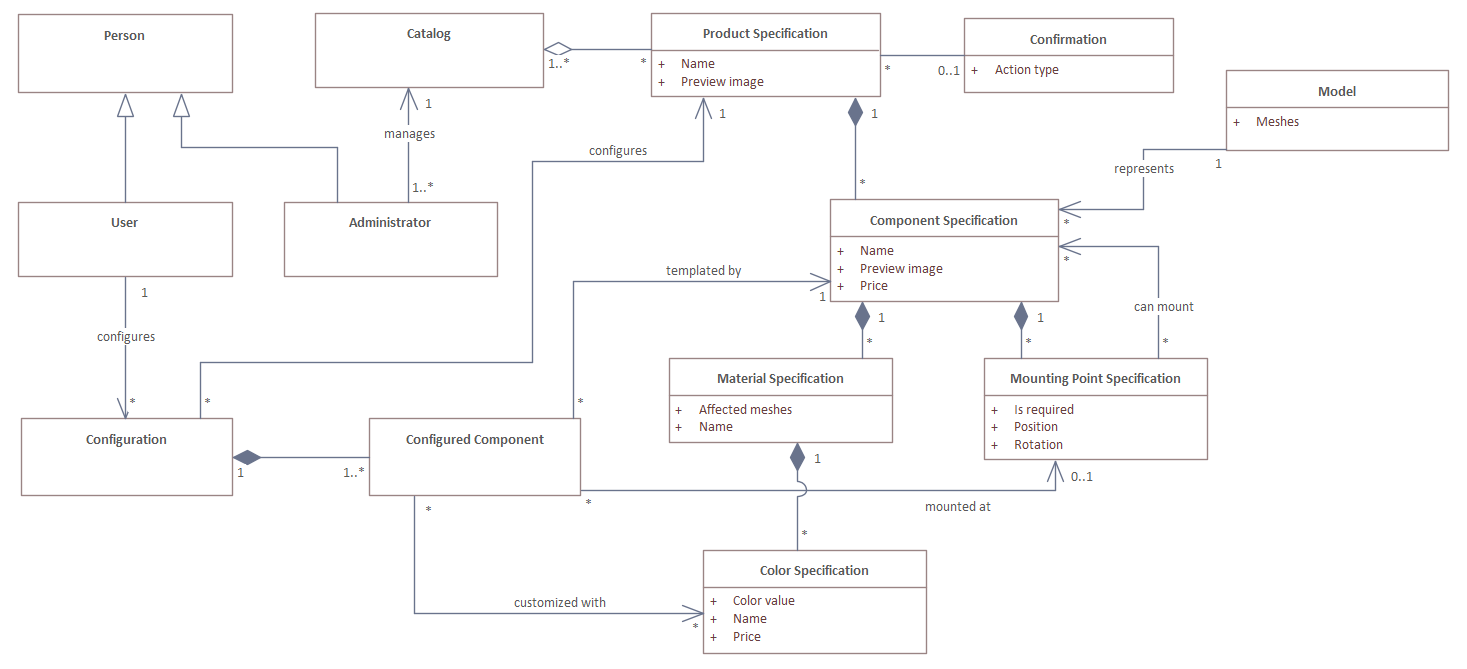
\includegraphics[width=\linewidth]{images/uml_domainmodel.png}
\caption{Domain model as a UML diagram}
\label{fig:domain-model}
\end{figure}
\end{landscape}

% - - - - - - - - - - - - - - - - - - - - - - - - - - - - - - -
\subsection{Catalog}
% - - - - - - - - - - - - - - - - - - - - - - - - - - - - - - -

The catalog forms the backbone of the proposed toolkit and defines the blueprint for customizable products. The catalog encompasses a variety of product specifications, each defining a configurable product along with all its potential customizations. This section delves into how these specifications lay the foundation for user-driven product configuration.
The entities discussed in this section are as follows:
\begin{itemize}[label=\rectanglebullet]
    \item Catalog
    \item Product Specification
    \item Component Specification
    \item Model
    \item Mounting Point Specification
    \item Material Specification
    \item Color Specification
    \item Administrator
\end{itemize}

A product specification acts as an overreaching comprehensive concept that encompasses all aspects of a given product. The entity may incorporate an action to finalize the configuration of the product, fulfilling the need for confirmation of the configuration (see requirement \hyperref[itm:F10]{F10}). Given that the tool focuses on the handling of modular products (see requirement \hyperref[itm:F3]{F3}), it is imperative that each product consists of various components. Therefore, the product specification is made up of component specifications, which represent all the various possible components that the product can have.

To meet the requirement of 3D visualization (see requirement \hyperref[itm:F3]{F3}), component specifications must be linked to a model featuring 3D meshes. This model acts as a representation of the component that will be presented to the user during the configuration process. In addition to this, the component specification is composed of material specifications and mounting point specifications.

Material specifications are needed with respect to the requirement of material color configuration (see requirement \hyperref[itm:F8]{F8}). They describe the materials of a given component that the user can customize, with each material specification providing mesh information specifying which part of the component this material influences, thereby enabling preview updates as the user makes selections. In addition, the material specification consists of color specifications that define the possible colors this material can take on in the configuration process.

Mounting point specifications are introduced to address the requirement of fixed point component placement (see requirement \hyperref[itm:F6]{F6}). They represent points on a component to which other modular components can be attached. The specifications of mounting point include the relative position and rotation of the point, the requirement for a component's presence at this point, and possible specifications of components that can be mounted on the point.

All these specifications are maintained in the catalog by the application administrator, who has the authority to modify any properties. The tool then utilizes these specifications to enable the configuration of tangible products.


% - - - - - - - - - - - - - - - - - - - - - - - - - - - - - - -
\subsection{Configuration}
% - - - - - - - - - - - - - - - - - - - - - - - - - - - - - - -

Transitioning from potential to actual, the configuration section delves into how users bring customizable products to life through the toolkit.
It illustrates how configured components are the building blocks of user-generated configurations, embodying the transformation from a generic template into a product uniquely tailored to individual preferences.
The entities covered in this section include:
\begin{itemize}[label=\rectanglebullet]
    \item Configuration
    \item Configured Component
    \item User
\end{itemize}

Users of the application create configurations. The cornerstone of a configuration lies in its configured components. The specifications described in the previous section serve as templates for these configured components. While the specifications outline all the configuration options, a configured component indicates a particular option selected by the user. Beyond the base component specification, a configured component also stores the mounting point to which it is attached, as well as the selected colors of its materials. Thus, a configuration is composed entirely of these individually configured components.


%______________________________________________________________
\section{User interface} \label{section:wireframes}
%---------------------------------------------------------------

The design of the user interface plays an essential part in the development of such a tool because it significantly influences user satisfaction when interacting with the tool. Good preparation of user interface design helps to determine the direction and streamline the implementation, as well as making clear from the beginning how to deal with factors such as responsiveness (see requirement \hyperref[itm:NF2]{NF2}).

In this section, low-fidelity wireframes are used to depict the proposed user interface, highlighting the layout and architecture of the application. This approach captures the most important information at this stage, leaving the finer details to be refined as part of the implementation phase.

The design is based on the analysis of existing solutions and respects the design principles of similar solutions that are most intuitive and the users may already feel familiar with.

The configurator as an application is specific in that it primarily centers around the configuration process, with this interface being the most important and all other interfaces being secondary. In this section, the design of this configuration screen will be introduced, as well as the introductory and confirmation screens.

The common element of all screens is the top bar with the logo of the business that operates the configurator, which should redirect the user to the main website of the company when clicked. All of this should be customizable in the admin settings of the application.

% - - - - - - - - - - - - - - - - - - - - - - - - - - - - - - -
\subsection{Configuration screen}
% - - - - - - - - - - - - - - - - - - - - - - - - - - - - - - -

\begin{figure}[h]
\centering
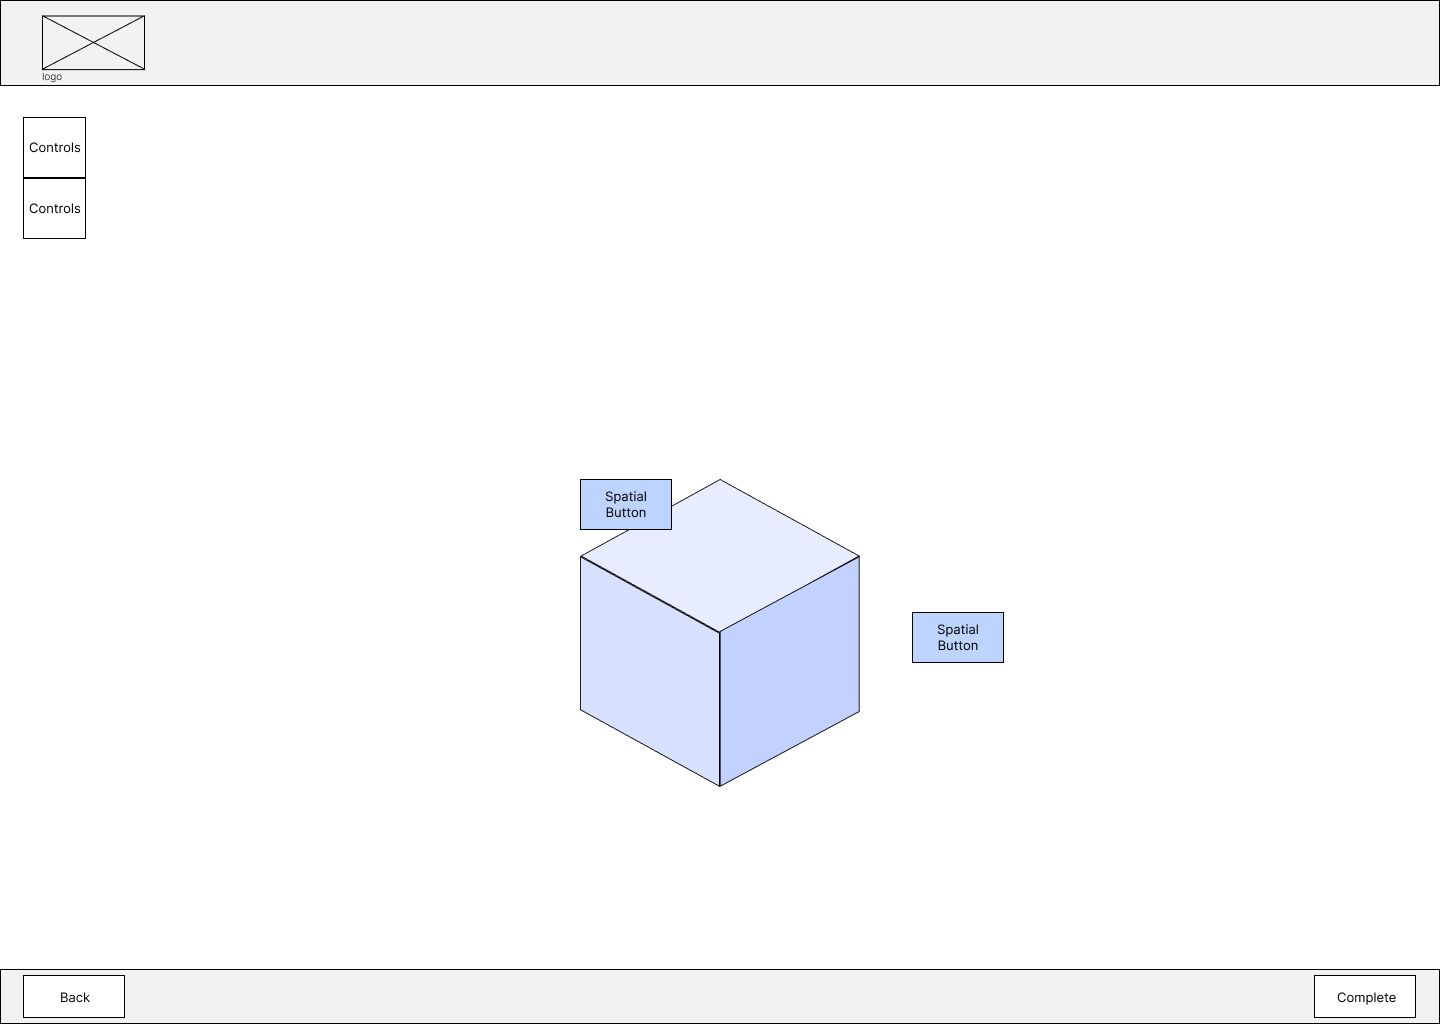
\includegraphics[width=0.7\textwidth]{images/wireframe_configuration_default.png}
\caption{Wireframe of configuration screen}
\label{fig:wireframe-configuration}
\end{figure}

The configuration screen is presented to the user during the configuration process. The screen is dominated by the 3D preview of the configured product, featuring interactable components and spatial buttons for the addition of components into the configuration. Control buttons are placed in the upper left corner within the 3D preview, symbolizing their direct relation to the preview, yet maintaining their distinctiveness as a separate element. At the bottom of the screen, there is another bar, this one containing buttons that allow users to go back or to finalize the configuration. The wireframe of the configuration screen in its default state is shown in  \autoref{fig:wireframe-configuration}, where the 3D preview of the product is represented by a blueish cube.

\begin{figure}[h]
\centering
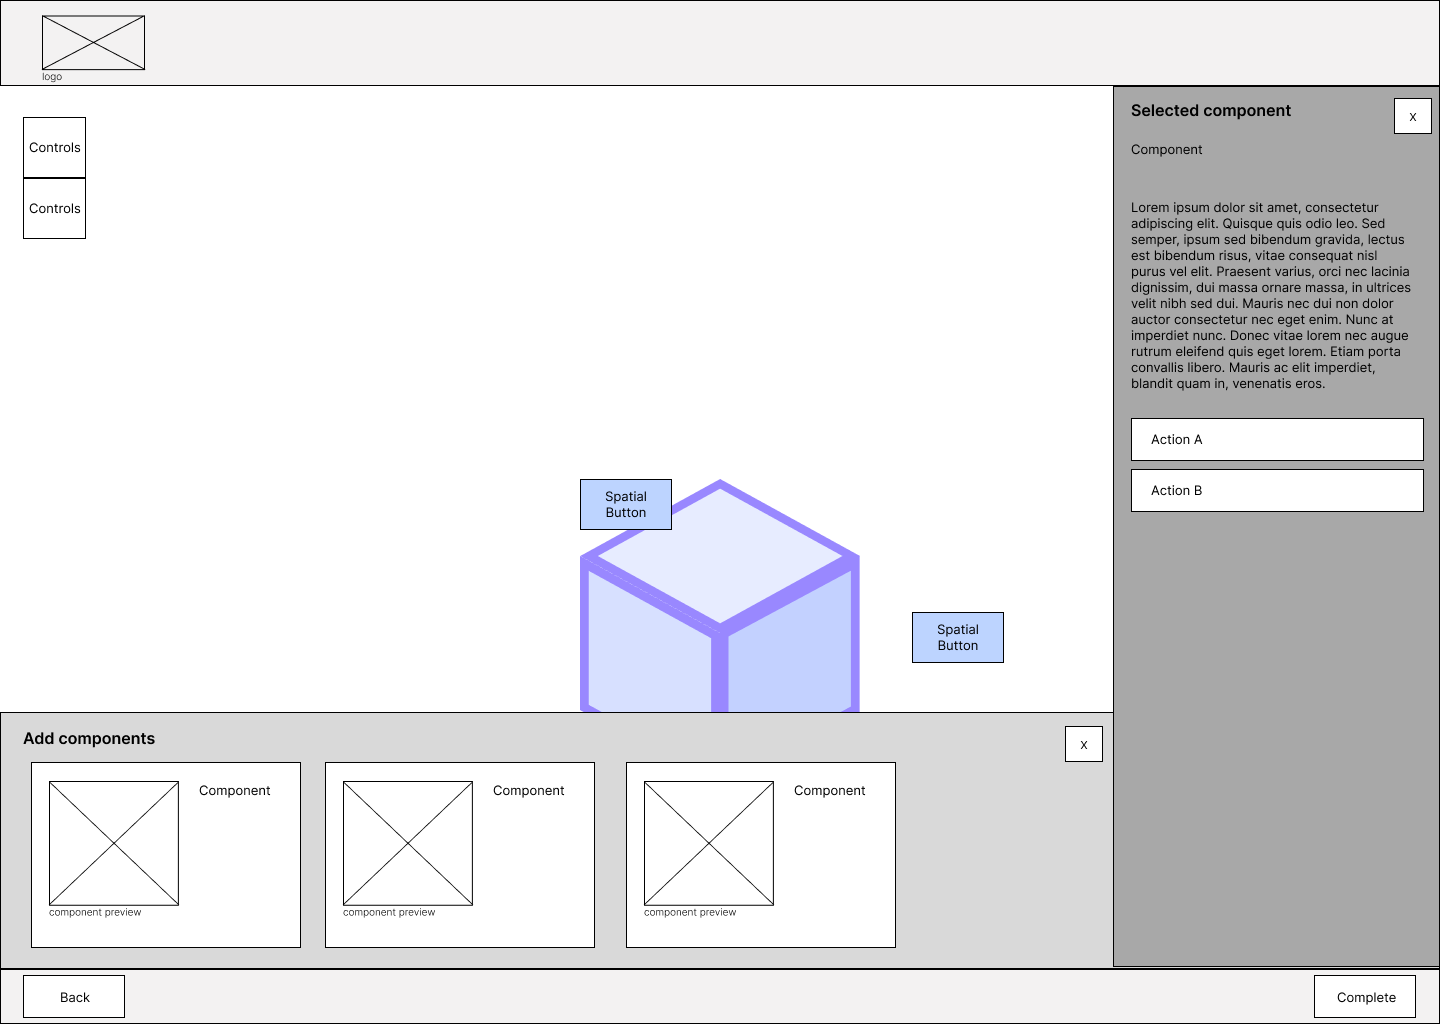
\includegraphics[width=0.7\textwidth]{images/wireframe_configuration_panels.png}
\caption{Wireframe of configuration screen with panels}
\label{fig:wireframe-configuration-panels}
\end{figure}

This default view, as outlined in the previous paragraph, maximizes the viewport with the most important presentation, which is the 3D preview of the product. However, at some stages of the configuration process, it is also necessary to present the user with further information. Therefore, upon selecting a component within the 3D preview, the component should become highlighted and, following the approach of existing solutions analyzed, a side panel with detailed information about the selected component will emerge from the right. If necessary, another panel with further options presented to the user may appear at the bottom. This design strategy maximizes the screen space for the important elements while still being flexible enough to present additional information in a streamlined way. The wireframe of the interface with panels that contain additional information and options presented is shown in \autoref{fig:wireframe-configuration-panels}.

\begin{figure}[h]
    \centering
    \begin{minipage}{0.4\textwidth}
        \centering
        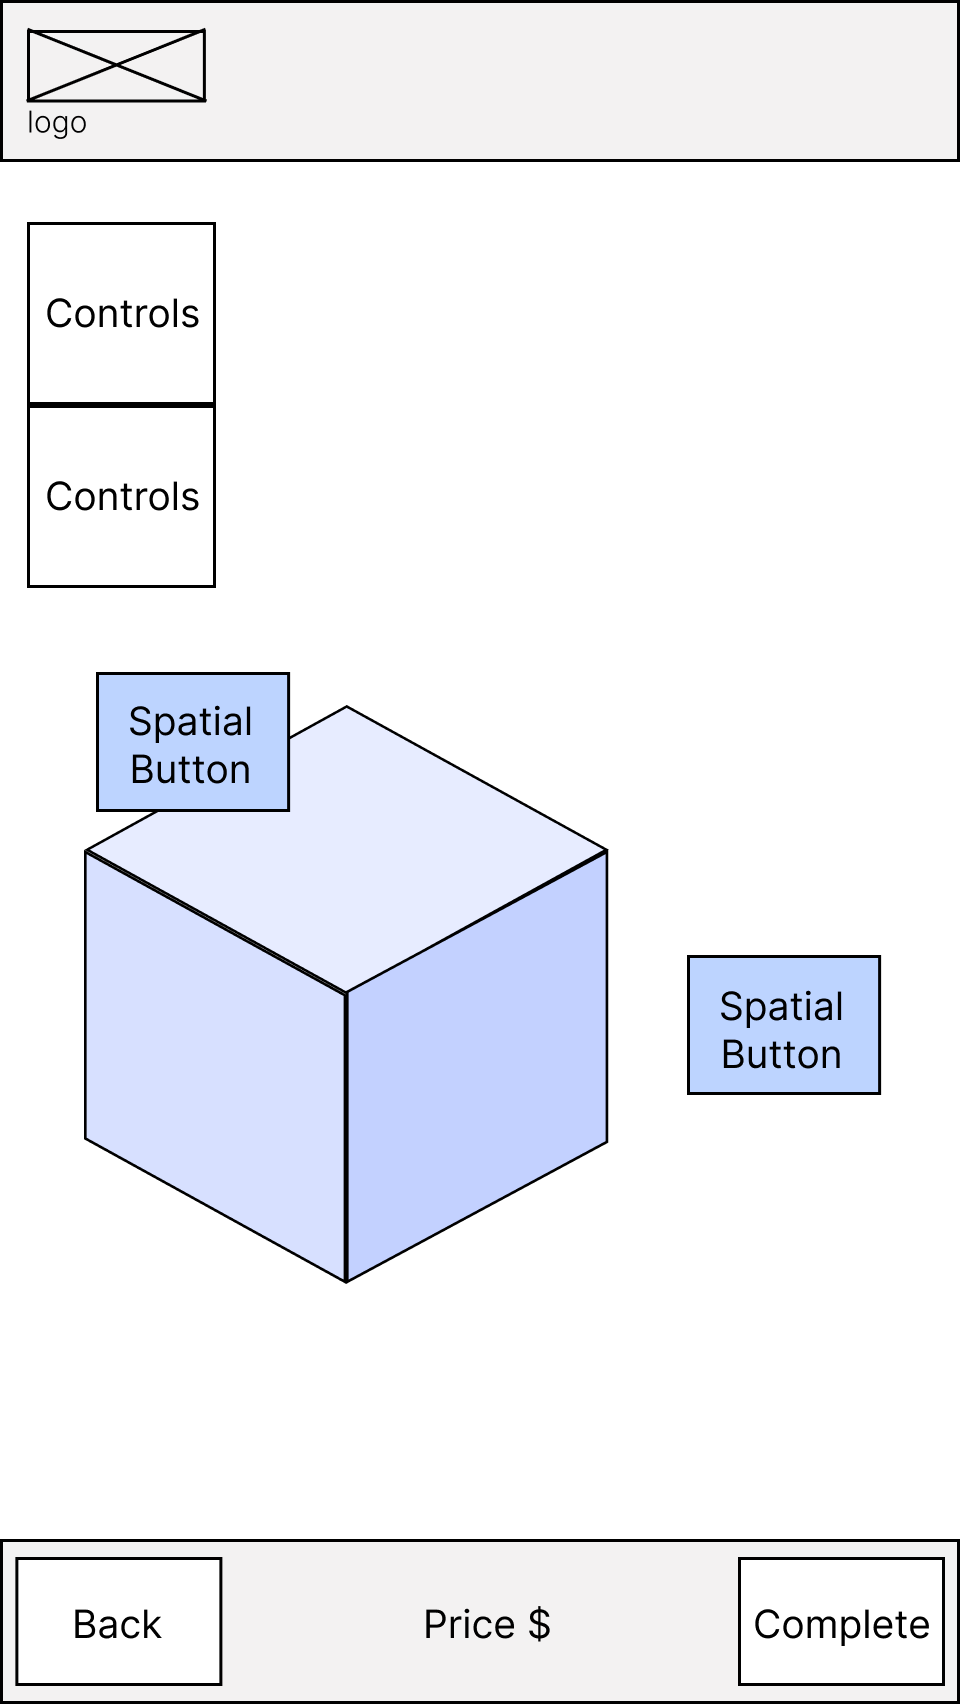
\includegraphics[width=\linewidth]{images/wireframe_configuration_mobile_default.png}
        \caption{Wireframe of mobile configuration screen}
        \label{fig:wireframe-configuration-mobile}
    \end{minipage}\hfill
    \begin{minipage}{0.4\textwidth}
        \centering
        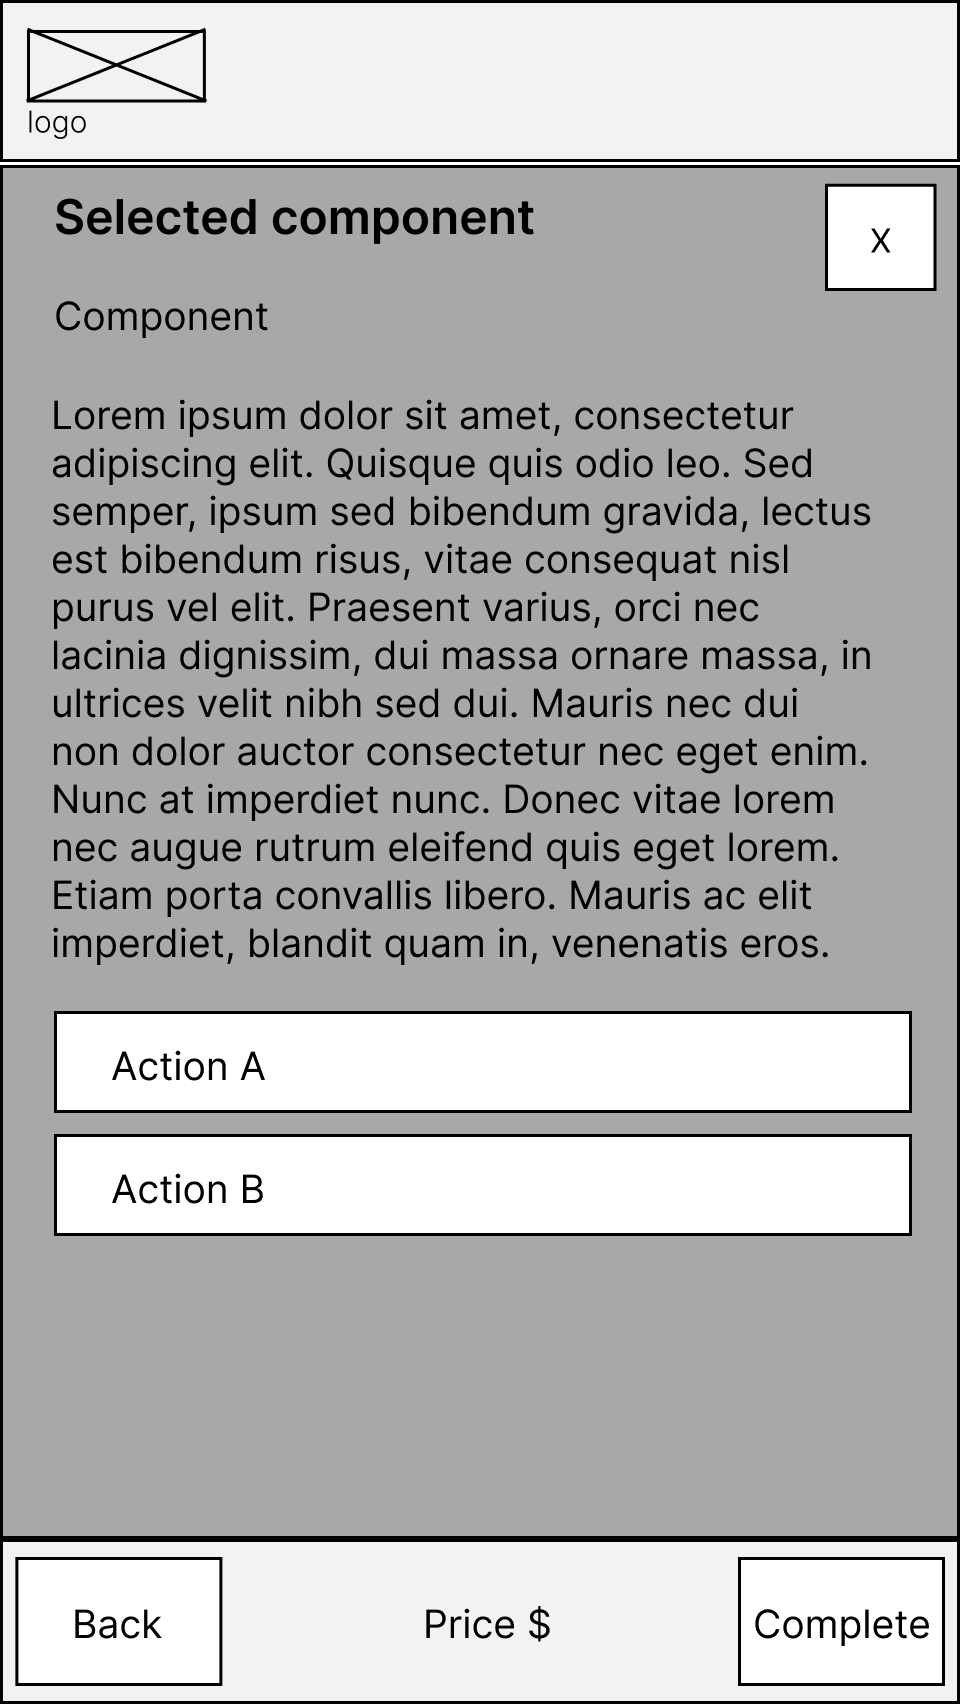
\includegraphics[width=\linewidth]{images/wireframe_configuration_mobile_panels.png}
        \caption{Wireframe of mobile configuration screen with panels}
        \label{fig:wireframe-configuration-panel-mobile}
    \end{minipage}
\end{figure}

To ensure responsiveness, a mobile version of the interface should also be outlined. The prioritization of the 3D preview in the default state makes this simple, as this just means that on smaller viewports the elements are presented in the same way, with the preview being in different aspect ratio, which is easily compensated by the 3D preview taking on different zoom level. The outline of this wireframe is presented in \autoref{fig:wireframe-configuration-mobile}.

The wireframe for the mobile version of the interface with the presented detail side panel is shown in \autoref{fig:wireframe-configuration-panel-mobile}. At this reduced viewport size, the side panel can maintain the same internal layout but to be usable it needs to occupy the whole 3D preview. This will need to be kept in mind when utilizing interactions with the 3D preview, as it may not always be fully visible when the panels are active. 

The design remains mostly consistent on both small and large viewports, while still being adaptive and responsive. This ensures that the familiarity with the tool is maintained for all viewport sizes.

% - - - - - - - - - - - - - - - - - - - - - - - - - - - - - - -
\subsection{Introduction screen}
% - - - - - - - - - - - - - - - - - - - - - - - - - - - - - - -

\begin{figure}[h]
\centering
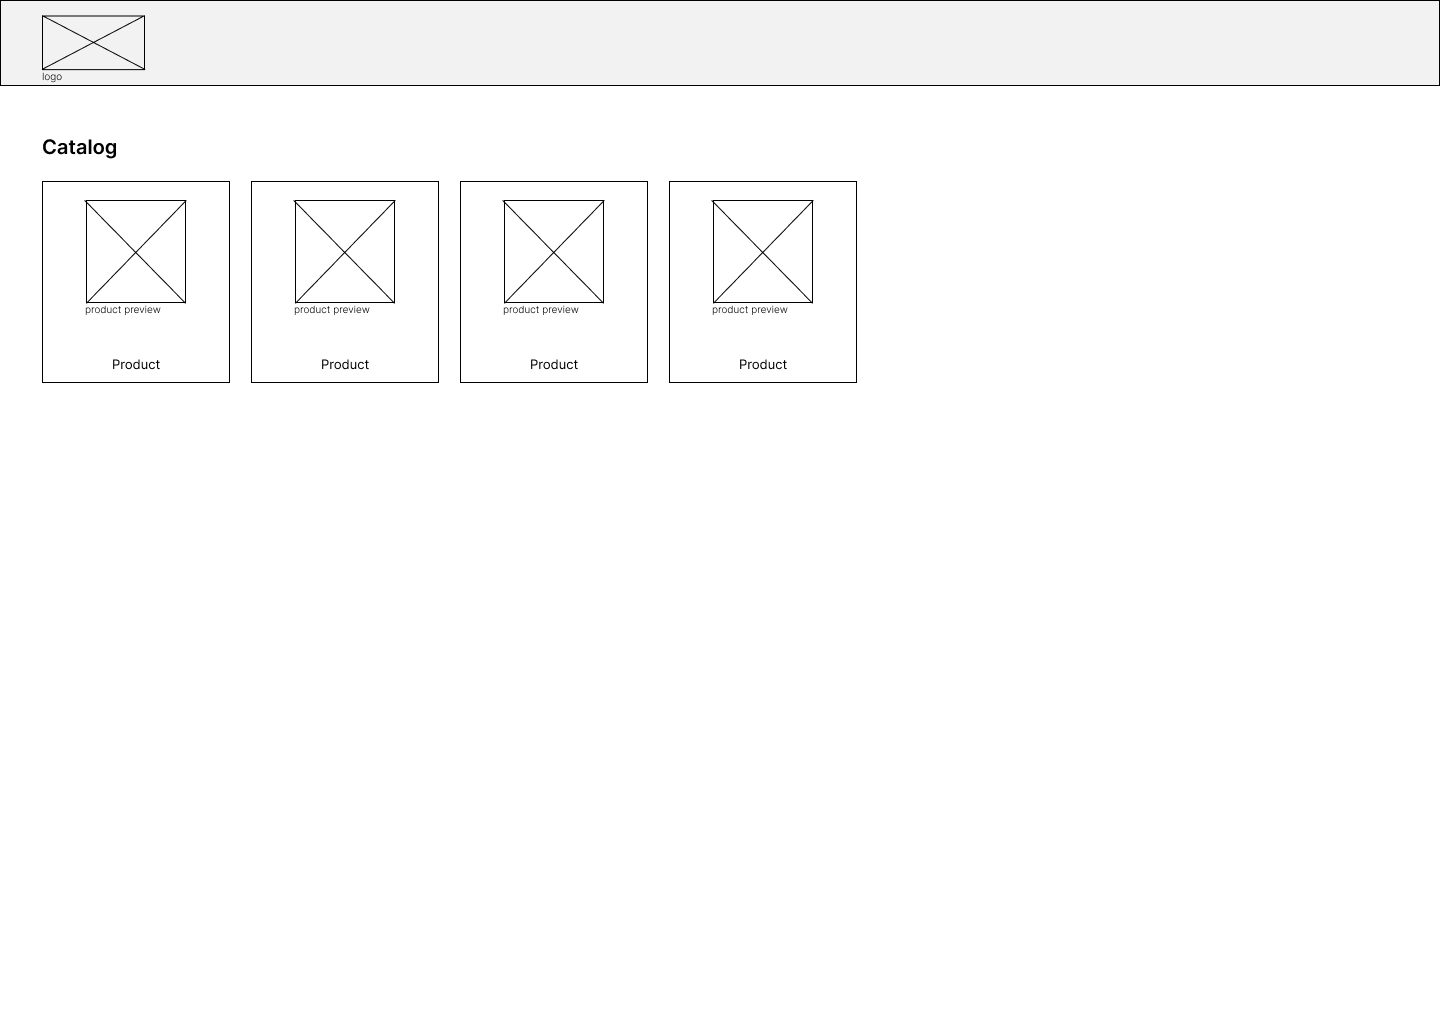
\includegraphics[width=0.7\textwidth]{images/wireframe_introduction_default.png}
\caption{Wireframe of introduction screen}
\label{fig:wireframe-introduction}
\end{figure}

The introduction screen is the first screen presented to the user when launching the application. It offers a simple way of selecting the configurable product from the catalog, with image and name of the product presented on a large tile. The selection of the product takes the user to the configuration process. Mobile interface of this screen mirrors the large version. The wireframe of the design can be seen in \autoref{fig:wireframe-introduction}.

% - - - - - - - - - - - - - - - - - - - - - - - - - - - - - - -
\subsection{Confirmation screen}
% - - - - - - - - - - - - - - - - - - - - - - - - - - - - - - -

\begin{figure}[hb]
\centering
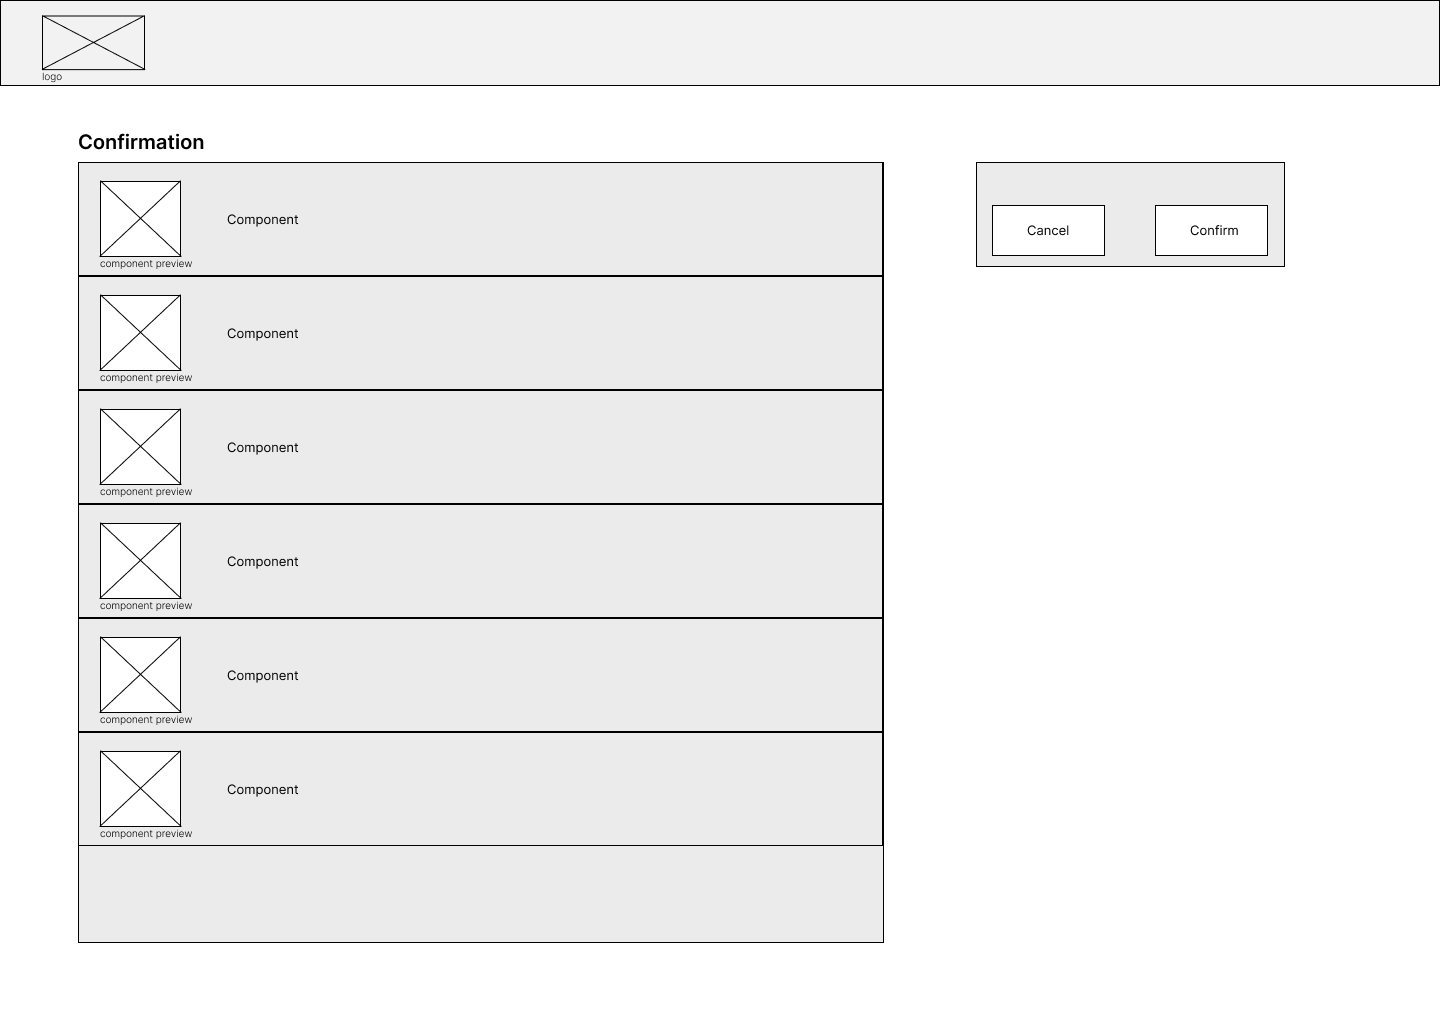
\includegraphics[width=0.7\textwidth]{images/wireframe_confirmation_default.png}
\caption{Wireframe of confirmation screen}
\label{fig:wireframe-confirmation}
\end{figure}

The confirmation screen is presented to the user at the end of the configuration and satisfies the configuration review requirement (see requirement \hyperref[itm:F9]{F9}). The wireframe of the configuration screen is shown in \autoref{fig:wireframe-confirmation}. On the left side, the confirmation screen presents the selected and configured components in a comprehensive list and allows the user to review their choices. The right side of the screen contains two buttons, one to confirm the configuration, which can initiate the confirmation action, and another to return to the configuration process for any adjustments. 

\begin{figure}[h]
\centering
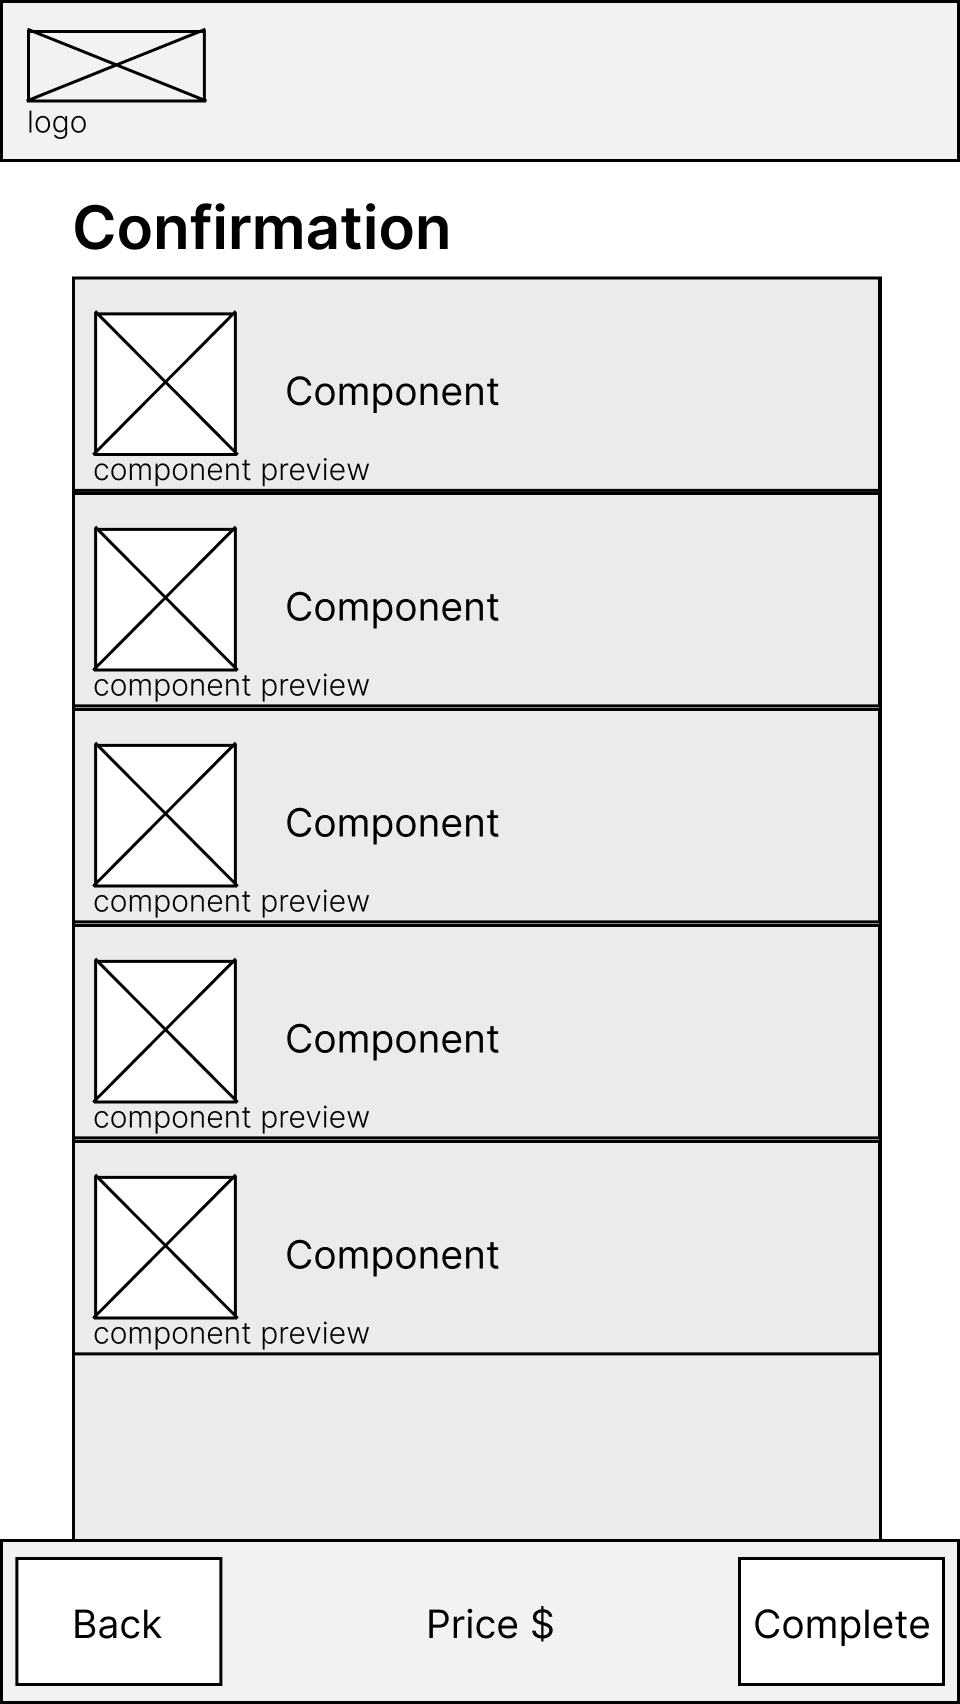
\includegraphics[width=0.3\textwidth]{images/wireframe_confirmation_mobile_default.png}
\caption{Wireframe of mobile confirmation screen}
\label{fig:wireframe-confirmation-mobile}
\end{figure}

The wireframe for the mobile version of the confirmation screen is depicted in  \autoref{fig:wireframe-confirmation-mobile}. In this layout, the summary spans the entire width of the screen, with the buttons moved to form a bar at the bottom of the screen.

\todo{Add prices to the wireframes and images and names to the domain model.}